\documentclass[a4paper]{article}
\title{\Huge{\textsc{Evolutionary Algorithms for Iterated Prisoner's Dilemma}}}
\usepackage[margin=3cm]{geometry}
\usepackage{graphicx}
\usepackage{wrapfig}
\usepackage{caption}
\usepackage{amsmath}
\usepackage{subcaption}
\usepackage[export]{adjustbox}
\usepackage{enumerate}
\usepackage{url}
\usepackage{authblk}
\usepackage{float}
\usepackage{wrapfig}
\usepackage{setspace}
\usepackage{mdframed}
\usepackage{booktabs}
\usepackage{ragged2e}

\def\changemargin#1#2{\list{}{\rightmargin#2\leftmargin#1}\item[]}
\let\endchangemargin=\endlist 

\DeclareMathSizes{10}{10}{10}{10}
\begin{document}

    \newgeometry{left=4cm,right=4cm,top=4cm,bottom=6cm}
	\begin{titlepage}
	    \begin{center}
	        \vspace*{1cm}
	        
	        {\huge{\textsc{Evolutionary Algorithms for Iterated Prisoner's Dilemma}}\\}
	        \vspace{8mm}
	        {\large{Nishant Rai}}\\
			\vspace{3mm}
			
			{\normalsize{Department of Computer Science and engineering\\}}
	        \vspace{4mm}
        	\vspace{7mm}
	        \textbf{Abstract\\}
        	\vspace{4mm}
        	\noindent
{\justifying{The project deals with the problem of computing successful strategies for Iterated Prisoner's dilemma. We propose multiple algorithms to compute good strategies which perform well against a set of baseline algorithms (Including the extremely simple yet effective 'Tit for Tat'). The proposed algorithms include Evolutionary Strategies and Reinforcement Learning to compute optimal and also adaptive strategies which perform well against multiple opponents. We discuss Axelrod's Tournament and use a similar setup to decide the effectiveness of the computed strategies. The result section shows the superiority of the strategies computed using them.} \par}
			\vfill
			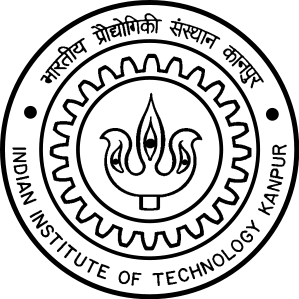
\includegraphics[width=0.25\textwidth]{iitklogo.png}\\[0.1in]
            \vspace{3mm}
            \normalsize{Under the guidance of Dr. Vimal Kumar\\}
            \vspace{1mm}
            {Indian Institute of Technology, Kanpur}
	    \end{center}
	\end{titlepage}
	\restoregeometry

	\tableofcontents
	
	\pagebreak	
	
	\section{Introduction}
	
	The Prisoner's Dilemma is a classic problem in game theory, discovered in 1950 by Melvin Dresher and Merrill Flood, whose purpose is, among other things, to describe a situation in which rational behavior (defined as that behavior which will maximize one's expected benefit) can be, in a sense, self-undermining. It has become a popular problem because it is seen as fundamentally similar to real-world problems in sociology and politics. \\
	The Prisoner's Dilemma can be described as follows: suppose that two individuals, A and B, have been arrested in connection with a crime. Each is put in a separate interview room and told that a deal may be available to them depending on whether each provides testimony against the other (defects) or keeps silent (cooperates). Each individual is assumed to want to do as well as possible for themselves without regard to the welfare of the other player.\\

	\tabcolsep=0.51cm
	\begin{table}[H]
	\centering
	\begin{tabular}{|c|c|c|}
	\hline
						& B co-operates            & B defects 					\\ \hline
	A co-operates  		& (3,3) 		 			& (0,5)         			\\ \hline
	A defects 			& (5,0)           			& (1,1)            			\\ \hline
	\end{tabular}
	\caption{Payoff matrix for the Prisoner's Dilemma}
	\end{table}
		
	\begin{table}[H]
	\centering
	\begin{tabular}{|c|c|c|}
	\hline
						& B co-operates            & B defects 					\\ \hline
	A co-operates  		& (R,R) 		 			& (S,T)         			\\ \hline
	A defects 			& (T,S)           			& (P,P)            			\\ \hline
	\end{tabular}
	\caption{State definitions for the Prisoner's Dilemma}
	\end{table}

	This situation is formally specified by the matrix in Figure 1, subject to the following definitions and restrictions:
	\begin{itemize}
		\item T : \textbf{Temptation} for unilateral defection
		\item R: \textbf{Reward} for mutual cooperation
		\item P : \textbf{Punishment} for mutual defection
		\item S: \textbf{Sacrifice} for unilateral cooperation	
	\end{itemize}
	
	A variant of the classical prisoner's game arises as a result of repeated games. It is termed as Iterated Prisoner's Dilemma. The situation is more interesting when the game satisfies the following conditions,
	\begin{enumerate}
	\item The number of moves should not be known to the two players.
	\item The winner is the player with the highest score in the end.
	\item Usually, there are many players in the fray, and there is a Round Robin Tournament among all the players - the player with the highest score wins.		
	\end{enumerate}
	
	\section{Existing Work}
	
	It can be argued that Axelrod has been the most influential researcher in the area of the Iterated Prisoner's Dilemma. In Axelrod's original work, two computer tournaments based on IPD were undertaken; which later defined the methods by which IPD strategies ought to be compared. In this process, Axelrod invited professional game theorists to submit programs for playing a computer-based Iterated Prisoner's Dilemma. Axelrod's work has also been extremely influential in other studies.\\
	Later, Axelrod used a Genetic Algorithm (GA), an artificial intelligence technique (Inspired by biological evolution), to simulate agent learning. The algorithm uses operators such as mutation and crossover (Derived from evolution). In investigating evolutionary future round tournaments, Axelrod considered a set of strategies that is deterministic and uses outcomes of the past 'three' moves (Discussed later) to determine a current move.\\
	Further works adapt the same approach. This means that all strategies encoded in these environments are history dependent. In other word, such environment consists only of memory-based strategies. However, alternative representation of strategies could exist. Kraines showed that ‘Pavlovian’ strategies are able to support the evolution of cooperation in tournaments where players are making errors. 
	
	\section{Axelrod's Tournament}

	In 1980, Robert Axelrod, professor of political science at the University of Michigan, held a tournament of various strategies for the prisoner's dilemma. He invited a number of well-known game theorists to submit strategies to be run by computers. In the tournament, programs played games against each other and themselves repeatedly. Each strategy specified whether to cooperate or defect based on the previous moves of both the strategy and its opponent.\\
	Some of the strategies submitted were:
	\begin{itemize}
	\item \textbf{Always Defect}: This strategy defects on every turn. This is what game theory advocates. It is the safest strategy since it cannot be taken advantage of. However, it misses the chance to gain larger payoffs by cooperating with an opponent who is ready to cooperate.
	\item \textbf{Always Cooperate:} This strategy does very well when matched against itself. However, if the opponent chooses to defect, then this strategy will do badly.
	\item \textbf{Random:} The strategy selects its move randomly i.e. cooperates and defects 50\% of the time.
	\end{itemize}
	
	All of these strategies are prescribed in advance. Therefore, they cannot take advantage of knowing the opponent's previous moves and figuring out its strategy. The winner of Axelrod's tournament was the 'Tit for Tat' strategy. The strategy cooperates on the first move, and then does whatever its opponent has done on the previous move. Thus, when matched against the all-defect strategy, 'Tit for Tat' strategy always defects after the first move. When matched against the all-cooperate strategy, 'Tit for Tat' always cooperates. This strategy has the benefit of both cooperating with a friendly opponent, getting the full benefits of cooperation, and of defecting when matched against an opponent who defects. When matched against itself, the 'Tit for Tat' strategy always cooperates.\\
	'Tit for Tat' relies on the assumption that its opponent is trying to maximize his score. When paired with a mindless strategy like 'Random', 'Tit for Tat' sinks to its opponent's level. For that reason, 'Tit for Tat' cannot be called a 'best' strategy. It must be realized that there really is no 'best' strategy for prisoner's dilemma. Each individual strategy will work best when matched against a 'worse' strategy. In order to win, a player must figure out his opponent's strategy and then pick a strategy that is best suited for the situation.
	
	\subsection{Features of Successful Strategies}

A strategy (pure) for a player in a particular game is a plan describing what move that player should take in each possible situation (information state) that might arise for him.
In Axelrod’s IPD tournaments, strategies exhibiting the following four properties tended to be more successful (i.e., to accumulate higher total payoffs), with the clear-cut winner being the Tit-for-Tat strategy.
	\begin{itemize}
		\item \textbf{Niceness}: Never be the first to defect.
		\item \textbf{Provocability}: Get mad quickly at defectors and retaliate.
		\item \textbf{Forgiveness}: Do not hold a grudge once you have vented your anger.
		\item \textbf{Clarity}: Act in ways that are straightforward for others to understand.
	\end{itemize}

	\subsection{Axelrod Strategies}	

As we have seen earlier that 'Tit for Tat', such a simple strategy turned out to be the winner in Axelrod's tournament. Axelrod set out to find other simple strategies with similar or greater power.\\
Axelrod adopted a simple but elegant way for encoding strategies, and then used a single-objective evolutionary algorithm to obtain optimal strategies. His encoding scheme remained a standard way of handling the IPD problem and is described below. We also adopt a similar encoding scheme to compute optimal strategies for the game. Axelrod's method had the following features,
	\begin{itemize}
	\item The next move depends upon the behavior of both the parties during previous three (In general k, termed as memory length in this paper) moves.
	\item We have four possibilities for the previous move, which are as follows,
	\begin{itemize}
		\item CC or R for Reward
		\item CD or S for Sucker
		\item DC or T for Temptation
		\item DD or P for Penalty
	\end{itemize}		
	\item We code the particular behavioral sequence as a 3-letter string.	
	\item We then use the 3-letter sequence to generated a number between 0 and 63 (i.e. $4^{3} = 4^{k}$) by interpreting it as an integer base 4 (Since there were 4 possibilities for each turn).
	\item Strategy string : 64-bit binary string of C's and D's where he $i^{th}$ bit corresponds to the $i^{th}$ behavioral sequence.
	\end{itemize}

	The following \textbf{critical} points should be observed,
	\begin{itemize}
	\item The behavior of the player is undefined in the first three moves of the game (Since we do not have histories of the game).
	\item We also add six bits to the encoding to specify a strategy's premises, i.e. assumption about the pre-game behavior.
	\item Together, each of the 70-bit strings represent a particular strategy (i.e. State-action codes)	
	\end{itemize}		
	
	\section{Motivation}
	
	As discussed in the previous section, Axelrod's encoding can be used to define a strategy. We decide to use Evolutionary Algorithms to compute the optimal (Axelrod) strategy because the total number of all possible strategies very high (i.e. $2^{70}$). If we perform exhaustive search, it will take a huge amount of time (A couple billion years or more!). We do not seek help from standard optimization procedure since the fitness function required is not continuous or differentiable, thus classical methods will not work. Hence, genetic (evolutionary) algorithms are a good choice.
	
	\section{Proposed Algorithms}
	
	\subsection{Axelrod Strategies using Evolutionary Algorithms}

	As mentioned earlier, Axelrod's approach involved maximizing the self score using a Single Objective Genetic Algorithm. We study Axelrod's model along with optimizing multiple objectives (i.e. Self Score and Opponent score) simultaneously using NSGA-II algorithm. We later compare the computed strategies.\\
	The intuition for using another objective (i.e. Opponent score) is that the Prisoner's dilemma game is similar to a constant sum game (If we exclude the case when both confess), thus minimizing the opponent score might indirectly help us in maximizing our own score.

	\subsection{Reinforcement Learning for Adaptive Strategies}
	
	\section{Experiments}
	
	Both Single Objective Evolutionary Algorithm and Multi Objective Evolutionary Algorithm (MEA) are used for getting optimal strategies. The proposed strategies are evaluated in the later sections as discussed below.\\
	We describe the rough structure of the evolutionary algorithms. In each generation, a certain number (referred to as population size) of strategies are generated, and each strategy was made to play against \textbf{n} other players. Each game consisted of \textbf{p} moves. Then the next generation is created using a recombination operator involving the best strategies from the earlier one. The payoff matrix is the same as shown in Table 1. The details of the \textbf{n} other players have been given in the section: \textit{Baseline Strategies}.

	\subsection{Baseline Strategies}
	
	The baseline strategies used in the experiments are as follows,
	\begin{enumerate}
	
	\item \textbf{Always Cooperate:} Cooperates on every move
	\item \textbf{Always Defect:} Defects on every move
	\item \textbf{Tit for Tat:} Cooperates on the first move, then simply copies the opponent's last move.
	\item \textbf{Suspicious Tit for Tat:} Same as Tit for Tat, except that it defects on the first move
	\item \textbf{Random:} Makes a random move.
	\item \textbf{Cyclic CCD:} Plays C, C, D periodically.
	\item \textbf{Tit for Two Tats:} Cooperates on the first move, and defects only when the opponent defects two times.
	\item \textbf{Soft Majority:} Begins by cooperating, and cooperates as long as the number of times the opponent has
cooperated is greater than or equal to the number of times it has defected, else it defects.
	\item \textbf{Hard Majority:} Defects on the first move, and defects if the number of defections of the opponent is greater than or equal to the number of times it has cooperated, else cooperates.
	\item \textbf{Hard Tit for Tat:} Cooperates on the first move, and defects if the opponent has defects on any of the previous three moves, else cooperates.
	\item \textbf{Prober:} Plays D, C, C initially. Defects forever if opponent cooperated in moves 2 and 3. Otherwise plays Tit for Tat.	
	\end{enumerate}
	
	\subsection{Tournament Setup}
	
	The tournament setup is inspired by Axelrod's initial study. It consists of a round robin tournament amongst all the strategies where each game is played for 200 turns. The whole tournament is repeated a few times (10 times in our experiments) to lessen the effect of randomness.

	\section{Results for Evolutionary Algorithm}

	\subsection{Evolution Statistics}

	\subsubsection{Single Objective Genetic Algorithm (Max-Avg Fitness)}	

	\begin{wrapfigure}{R}{0.55\textwidth}
	\centering
	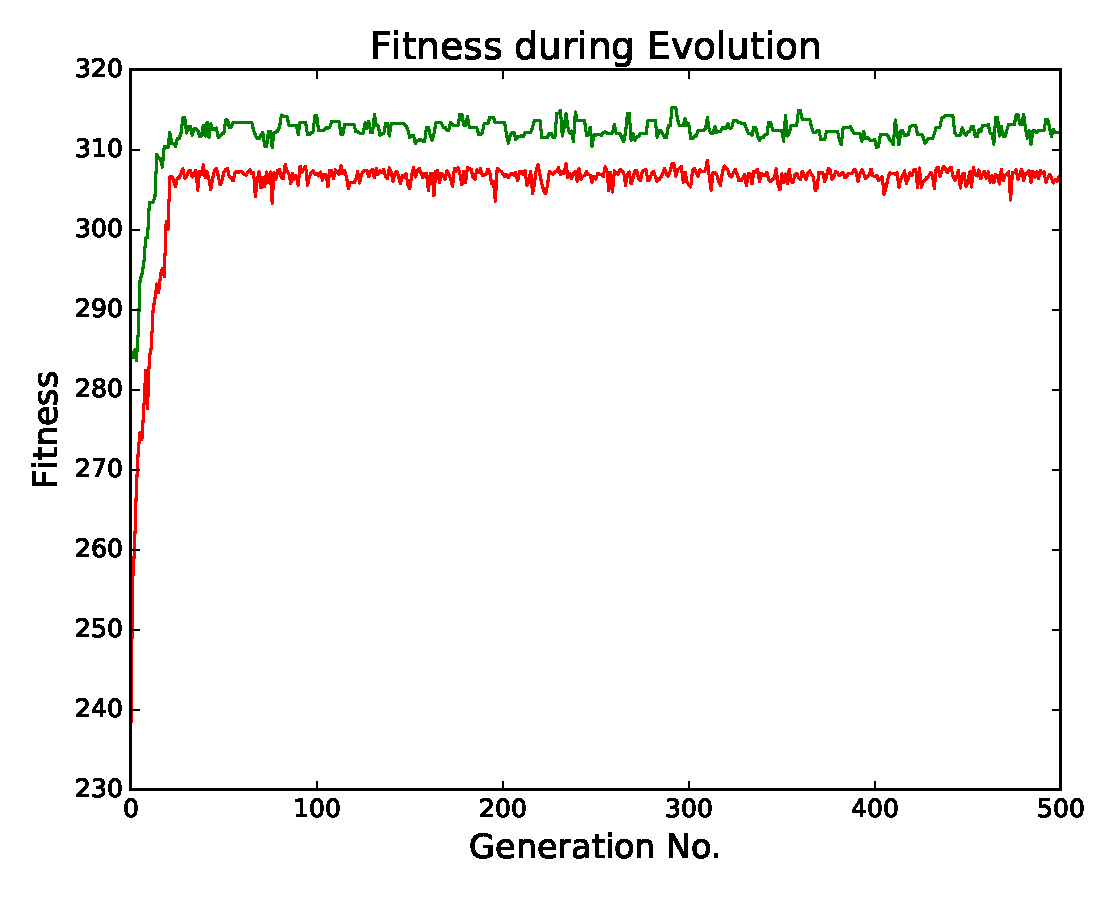
\includegraphics[width=0.53\textwidth]{singFitPlot.eps}
	\caption{\footnotesize{Fitness of Population during Evolution}}
	\end{wrapfigure}
	The single-objective Evolutionary Algorithm used is the same as used by Axelrod in his initial study. As done earlier, the fitness i.e. self-score of the player is maximized during evolution. For the experiment, the population size was fixed at 60. The results obtained when the evolutionary algorithm is run for 500 generations is shown in figure.\\
	We show the maximum and average fitness of the population. As we can see the population achieves the final value extremely quickly (Under 50 iterations). The fluctuations caused in between are a result of the mutations introduced in the population (Something inherent in Evolutionary Algorithms).\\
	After 500 generations the maximum fitness amongst all the samples in the population is around 312, which is even higher than the benchmark score (300) \textbf{(Dawkins)}. This shows the superiority of the Evolutionary strategy and is also in line with the results obtained by Axelrod. When this strategy is pitted against other strategy in an Axelrod-like tournament, the evolved strategy emerges as a clear winner (By a huge margin). The results are discussed in later sections.	

	\subsubsection{Multi Objective Genetic Algorithm (Max-Avg Fitness)}
		
	\begin{wrapfigure}{R}{0.55\textwidth}
	\centering
	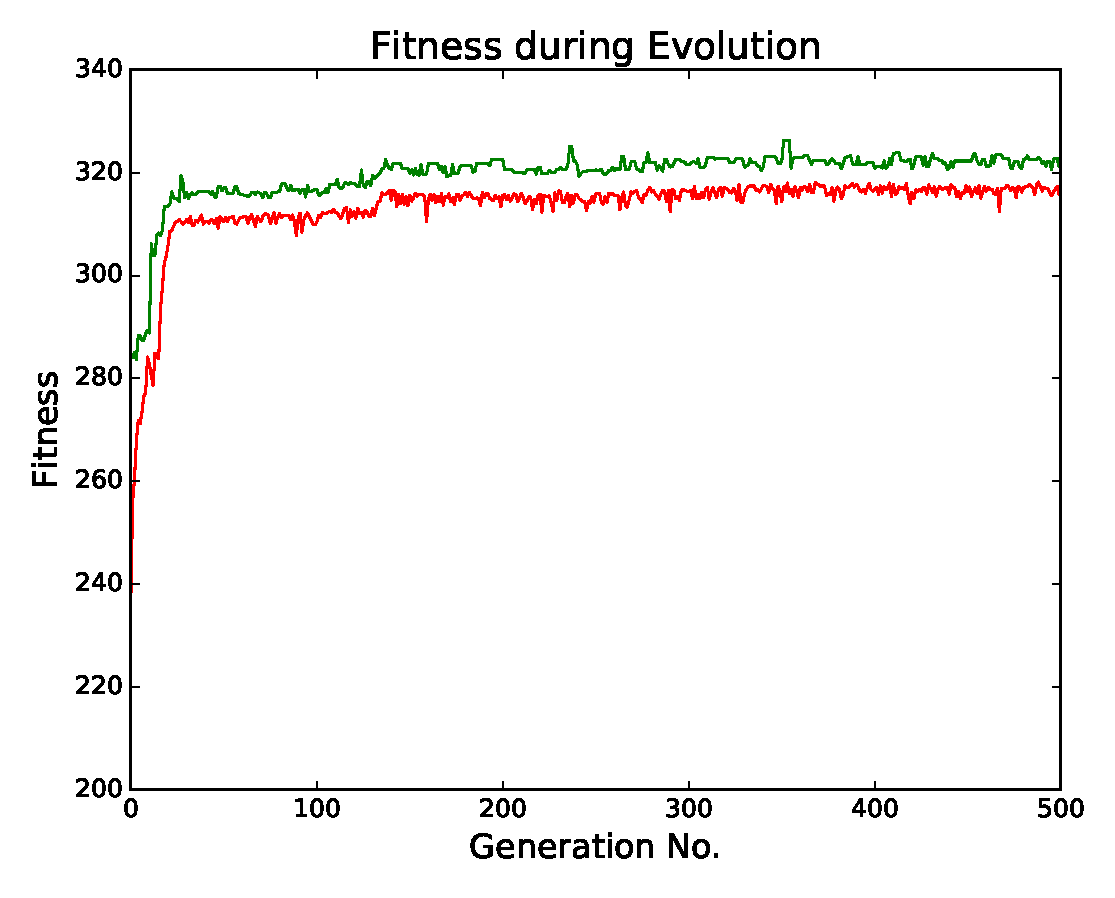
\includegraphics[width=0.53\textwidth]{multFitPlot.eps}
	\caption{\footnotesize{Fitness of Population during Evolution}}
	\end{wrapfigure}
	Instead of just maximizing our own score as proposed by Axelrod, we perform another experiment in which along with maximizing our self score we also try to reduce the opponents score. The intuition for this can be seen from the payoff matrix of the game. Assume that the opponent has selected his move and it's our turn to choose. Notice that for all moves of the opponent, the one in which we get higher payoff is the one in which our rival gets a lower payoff.\\
	We used a Multi-Objective Evolutionary Algorithm (NSGA-II) to compute the strategy. For the experiment, the population size was fixed at 60. The results obtained when the evolutionary algorithm is run for 500 generations is shown in figure. We show the maximum and average fitness of the population. The behavior of evolution mostly remains similar to the previous case. But we can see that the final value obtained \textit{(321)} in this case is higher than the Single Objective counterpart \textit{(312)}, which further motivates the benefit of using a multi-objective optimization algorithm.\\

	To further demonstrate the evolution, we plot the initial and final strategies obtained in Figure 3. The blue crosses represent the initial randomly initialized strategies. The red pluses represent the final evolved strategies, it can be easily seen that the initially random population slowly approaches the 'optimal' region. The out of place red members in the final evolved population are the mutated individuals.

	\begin{figure}[H]
	\centering
	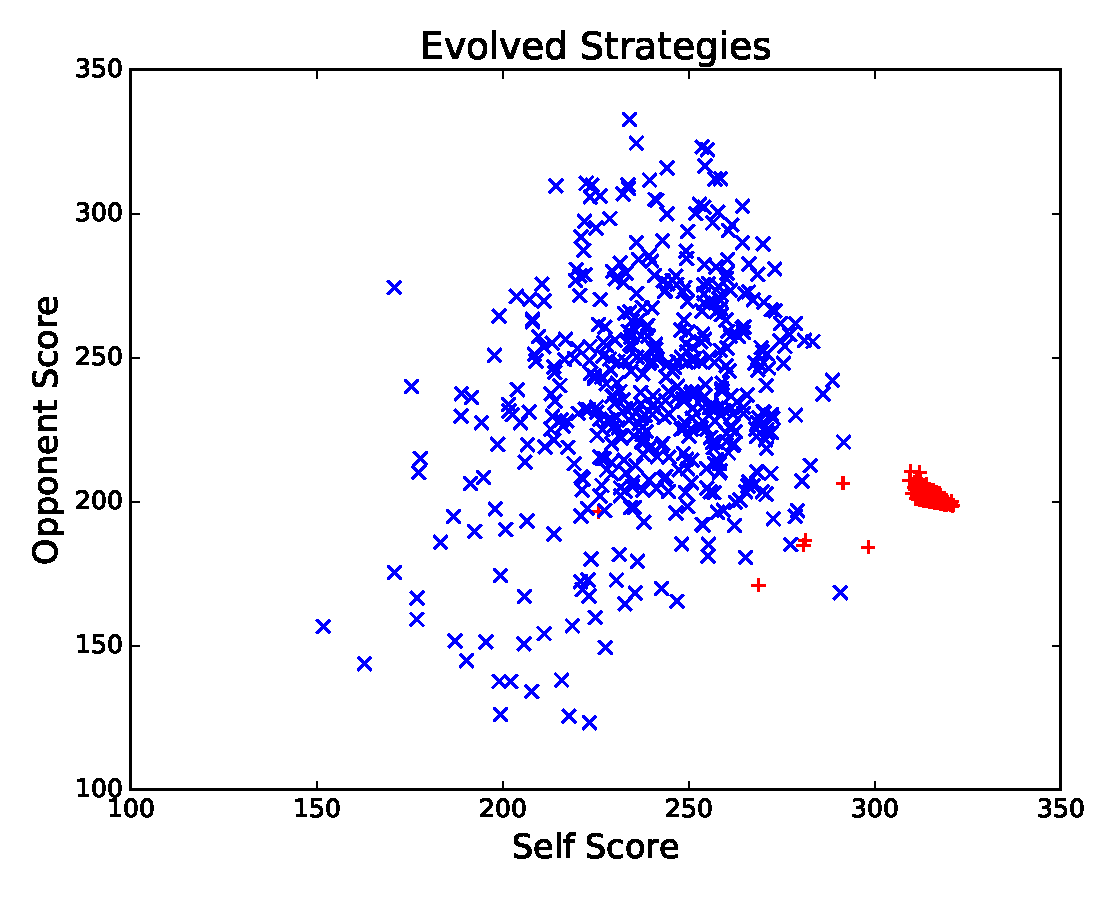
\includegraphics[width=0.75\textwidth]{evolvePlot.eps}
	\caption{{Distribution of Final Evolved Strategies and the Initial Randomly initialized Strategies}}
	\end{figure}

	\subsection{Plotting Optimal strategies}

	\subsection{Effect of Memory on Strategies}
	
	\textbf{Fitness vs Memory Used}\\
	\textbf{Computation Time vs Memory Used}
	
	\subsection{Tournament amongst strategies}
	
	\subsection{Observations}

	\subsubsection{Similarities between Optimal strategies}
	
	\subsubsection{Effect of Memory on Strategies}	

	\section{Results for Adaptive Strategies}

	\subsection{Learning Performance}
		
	\subsubsection{Performance Against Other Strategies}
	\subsubsection{Initial Behavior (Payoff)}
	\subsubsection{Behavior in the Long-run}

	\subsection{Observations}
	
	\subsubsection{Effect of Parameters on Learning}
	\subsubsection{Effect of Memory}
	\subsubsection{Special Cases: Cooperator and Defector}

	\section{Showdown: Evolved Strategy Vs Adaptive Strategy}

	\subsection{Performance Against Each Other}
	\subsection{Performance Against Other Strategies}

	\section{Future Work}
			
	\section{References}

\end{document}


